\section{Implementazione}
Uno degli obiettivi principali del progetto \emph{PathS} è di fornire indicazioni di navigazione ai suoi utenti. Si è quindi presentata la necessità di dover rispondere a quesiti di \emph{routing} utilizzando le informazioni raccolte tramite le operazioni di campionamento e l'interrogazione del servizio di cartografia. 

Allo scopo di agevolare l'implementazione del componente e di ottimizzare le operazioni di calcolo è stata selezionata per l'utilizzo la libreria \emph{PGRouting} la quale fornisce un grande supporto in questo senso. Questa estensione si appoggia alle funzioni \emph{GIS} del database, introducendo le capacità di calcolo del percorso tramite l'utilizzo di algoritmi generici già implementati e configurabili ad esempio Floyd-Warshall, Shortest Path A*, Dijkstra e \emph{Traveling Sales Person}.

Tuttavia per poter operare correttamente la libreria necessita che siano verificate alcune precondizioni sulla base dati da utilizzare, in particolare:
\begin{itemize}
	\item la rete di trasporto deve contenere informazioni corrette in corrispondenza delle intersezioni e degli estremi dei tratti adiacenti;
	\item la base dati deve contenere le informazioni sulla topologia della rete affinché si possa costruire un grafo utilizzabile dagli algoritmi.
\end{itemize}

Per affrontare il primo problema, la libreria mette a disposizione una funzione di ``\emph{noding}''. Tale procedura riceve in input la tabella in cui sono contenuti i dati geografici e un valore di tolleranza, quindi rielabora le informazioni cercando di rimuovere situazioni non coerenti ad esempio:
\begin{itemize}
 \item intersezioni non gestite come il caso \emph{(1)} in figura \ref{fig:pgrouting-noding}. In alcuni casi i segmenti presenti nel database potrebbero intersecarsi senza però che sia presente il corrispondente punto di intersezione. In questa situazione le successive operazioni di \emph{routing} non sarebbero in grado di sfruttare l'intersezione come punto di svolta. La procedura quindi analizza i dati \emph{GIS} per individuare le possibili sovrapposizioni e in corrispondenza delle stesse crea dei vertici aggiuntivi spezzando i segmenti. La procedura mantiene traccia del numero e dell'ordine in cui vengono decomposti gli elementi originali.
 \item segmenti adiacenti con estremi che non coincidono come il caso \emph{(2)} in figura \ref{fig:pgrouting-noding}. In questa situazione la funzione cerca di semplificare e riunire in un unico vertice gli elementi che sono all'interno della distanza di tolleranza impostata. Senza questa elaborazione i due segmenti non potrebbero essere utilizzati dall'algoritmo di \emph{routing} dato che non sono comunicanti.
\end{itemize}

\begin{figure}[ht]
  \centering
  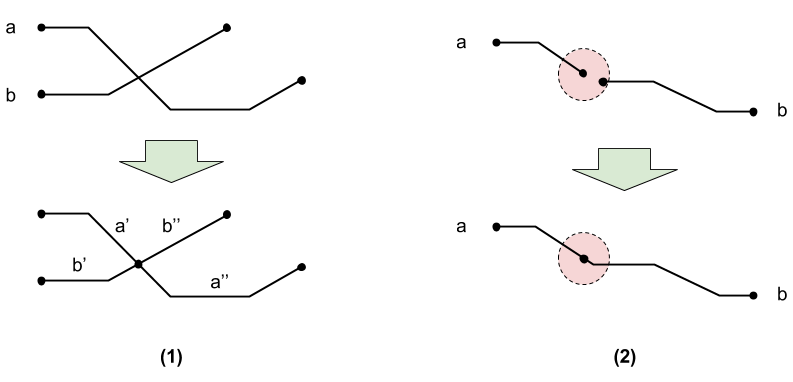
\includegraphics[width=.8\textwidth]{pgrouting-noding}
  \caption{\footnotesize{Casi in cui si applica la procedura di \emph{noding}.}}
  \label{fig:pgrouting-noding}
\end{figure}

Nel caso del database di \emph{PathS} la procedura di \emph{noding} viene eseguita sulla tabella \texttt{roadsegment} e il risultato è salvato nella tabella \texttt{roadsegment\_noded}. La procedura non altera i dati originali, ma è necessario rilanciarla ogni volta che si aggiungono nuovi elementi all'insieme dei segmenti importati tramite il servizio di cartografia.

Le informazioni dei segmenti rielaborate tramite la procedura di \emph{noding} possono essere quindi utilizzate per generare il grafo della rete di trasporto, sul quale saranno lanciati gli algoritmi di routing. L'operazione di generazione del grafo è implementata da un'altra funzione messa a disposizione dalla libreria, ovvero: \texttt{pgr\_createTopology}. In modo simile alla precedente, la funzione riceve come argomenti il nome della tabella da cui leggere le informazioni geografiche dei segmenti e un valore di tolleranza entro il quale eseguire l'operazione di unificazione dei tratti non connessi. Il risultato, nel caso specifico, porta alla generazione della tabella \texttt{roadsegment\_noded\_vertices\_pgr}. 

La struttura della tabella utilizzata per la persistenza delle informazioni dei segmenti e le conseguenti elaborazioni è presentata in figura \ref{fig:db-segments}.
\begin{figure}[ht]
  \centering
  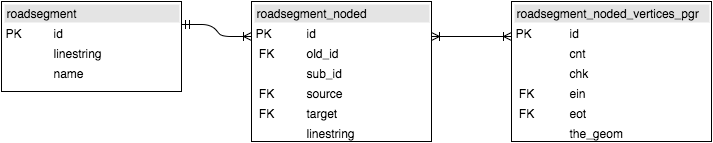
\includegraphics[width=\textwidth]{db-segments}
  \caption{\footnotesize{Schema tabelle relative ai segmenti della rete di tasporto.}}
  \label{fig:db-segments}
\end{figure}

Eseguite le operazioni di pre-processamento, i dati a sistema sono nella forma corretta per poter essere utilizzati dagli algoritmi di routing della libreria \emph{PGrouting}. A supporto dell'utilizzo e interpretazione del risultato è stata implementata la classe \texttt{app.utils.RouteResult} e le operazioni da eseguire sono state riunite nel metodo \texttt{getRouteResultFromQueryResult()}.

\section{Percorsi calcolati}
\subsection{Shortest Path}
La prima tipologia di percorso che si è deciso di calcolare è stato il caso semplice del percorso più breve (\emph{Shortest Path}). In questo modo è stato possibile valutare l'effettiva funzionalità della libreria e correggere eventuali errori nella procedura.
L'algoritmo adottato per il calcolo è quello di \emph{Dijkstra} implementato dalla funzione \texttt{pgr\_dijkstra}. Le modalità richieste per l'invocazione dell'algoritmo richiedono come argomenti:
\begin{itemize}
\item il nodo sorgente da cui inizia il percorso, specificato tramite \emph{id} così come è presente nella tabella dei vertici;
\item il nodo destinazione del tragitto, anch'esso individuato tramite \emph{id};
\item una \emph{query} con la quale ricavare i costi per ciascun arco del grafo della rete di trasporto.
\end{itemize}
Per identificare i nodi sorgente e destinazione, il server esegue una ricerca a database calcolando i vertici più vicini rispetto alle coordinate di latitudine e longitudine fornite. 

Per quanto riguarda il costo da utilizzare per ciascun arco, trattandosi del semplice caso \emph{Shortest Path}, si è svilupata una \emph{query} che ritorna come valore la lunghezza in metri del segmento stesso. L'algoritmo di \emph{routing} cercherà quindi di minimizzare il peso degli archi selezionati e quindi il tragitto più breve.

Il risultato dell'interrogazione è manipolato tramite la classe di utilità \texttt{RouteResult} per ricavare alcune informazioni aggiuntive come ad esempio la lunghezza totale del percorso o le indicazioni di svolta tra un tratto di strada e il successivo. 

Il modo in cui si presentano i dati all'applicazione client ma anche al browser web è stato scelto coerentemente con le altre \emph{API}; anche in questo caso si è optato per una risposta in formato \emph{GeoJSON} ed un esempio di invocazione è riportato in \ref{response-routing}.

\begin{lstlisting}[caption=Invocazione API di routing,label=response-routing]
GET /api/route?

BODY: 
{
    "type": "FeatureCollection",
    "features": [
        {
            "type": "Feature",
            "geometry": {
                "type": "LineString",
                "coordinates": [
                    [
                        11.8882108,
                        45.4107728
                    ],
                    ...
                    [
                        11.8917144,
                        45.409708
                    ]
                ]
            },
            "properties": {
                "comment": "Shortest Path - generato con PGRouting",
                "color": "red",
                "distance": 388.26767042966577,
                "maneuvers": [
                    {
                        "narrative": "Parti da Passeggiata Arturo Miolati",
                        "iconUrl": "/public/images/start.gif",
                        "streets": [
                            "Passeggiata Arturo Miolati"
                        ]
                    },                  
                    ...
                    {
                        "narrative": "Svolta a sinistra in Via Leonardo Loredan",
                        "iconUrl": "/public/images/left.gif",
                        "streets": [
                            "Via Leonardo Loredan"
                        ]
                    },
                    {
                        "narrative": "Sei arrivato a destinazione",
                        "iconUrl": "/public/images/end.gif",
                        "streets": [
                            "Via Leonardo Loredan"
                        ]
                    }
                ],
                "maneuverIndexes": [
                    0,             
                    ...
                    9
                ]
            }
        }
    ]
}
\end{lstlisting}

L'interpretazione della stessa risposta avviene con modalità diverse nei sistemi client, ovvero:
\begin{itemize}
\item nella applicazione mobile viene attivata la modalità di navigazione e le indicazioni \emph{turn-by-turn};
\item nel browser si presenta il percorso completo sulla vista mappa segnalando la lunghezza totale e un riassunto delle indicazioni di svolta.
\end{itemize}

\subsection{Percorsi con \emph{label}}
Uno degli obiettivi principali del progetto \emph{PathS} è il calcolo del percorso sfruttando le informazioni ricevute dai campionamenti di luce e rumorosità. L'implementazione dell'algoritmo di \emph{routing} per questo caso utilizza la stessa procedura presentata al punto precedente, manipolando però le strutture dati in moda da utilizzare le informazioni aggiuntive relative alle \emph{label}.

Le problematiche da risolvere in questo contesto sono state principalmente due:
\begin{itemize}
\item introdurre la gestione del contesto \textbf{temporale} in cui viene eseguita l'interrogazione così come per i dati da interrogare. Mentre per il caso semplice \emph{Shortest Path} si fa riferimento ad informazioni immutabili nel tempo, in questo caso un'interrogazione in momenti diversi della giornata può comportare alla consultazione di dati diversi e quindi risultati diversi;
\item modificare la logica di \textbf{calcolo dei pesi} introducendo la valutazione dei campioni a sistema, in un modo coerente e funzionale con gli obiettivi di \emph{routing}. 
\end{itemize}
Per gestire il primo problema, si è proceduto con il definire il concetto di \textbf{classe temporale}. Tutti i campioni ricevuti sono stati suddivisi, sulla base del \emph{timestamp} della rilevazione stessa, in insiemi distinti che rappresentano una fascia oraria delle giornata. Come compromesso tra semplicità e acuratezza dei risultati, si è scelto di definire quattro classi temporali uniformi, ciascuna delle quali copre un intervallo di 6 ore. Rispettivamente:
\begin{itemize}
\item classe \texttt{\textbf{0}} dalle \texttt{00:00} alle \texttt{05:59}: rappresenta il periodo notturno in cui i campioni di luminosità dovrebbero essere praticamente nulli così come quelli di rumorosità dovrebbero presentare valori molto bassi;
\item classe \texttt{\textbf{1}} dalle \texttt{06:00} alle \texttt{11:59}: rappresenta il periodo influenzato delle condizioni di luce mattutine così come dalle attività (es. traffico pendolare);
\item classe \texttt{\textbf{2}} dalle \texttt{12:00} alle \texttt{17:59}: è la fase in cui i campionamenti di luce dovrebbero essere determinanti data la maggiore esposizione;
\item classe \texttt{\textbf{3}} dalle \texttt{18:00} alle \texttt{23:59}: è l'intervallo temporale serale, in cui la luce rilevata torna ad essere meno influente mentre i campionamenti audio potrebbero essere influenzati da attività particolari (es. traffico, attività di intrattenimento)
\end{itemize}
Per agevolare l'attribuzione dei campioni alla relativa classe temporale in tutte le operazioni a database, è stata definita una funzione di utilità così come consentito dal database \emph{PostgreSQL}. La definizione della funzione è \texttt{time\_class(timestamp without timezone) $\rightarrow$ integer} la quale riceve in input il timestamp del campione e ritorna l'intero della classe temporale di appartenenza. Accentrando in un unico punto l'operazione di assegnazione, risulterà più agevole, se fosse necessario, cambiare le regole da utilizzare. 

Un'altra operazione a supporto della manipolazione dei dati per questo caso di \emph{routing} è stata la definizione di alcune viste a database le quali riassumono le informazioni relative ai campionamenti e le presentano in una forma più agevole per lo sviluppo delle query. Le viste implementate sono \texttt{light\_sample} e \texttt{noise\_sample} la cui struttura è presentata in figura \ref{fig:db-views}. In questo modo si riassumono in un unico punto le informazioni complete relative ad un campionamento, ovvero:
\begin{itemize}
\item l'\textbf{id} di riferimento;
\item il \textbf{segmento} della rete di trasporto a cui è stato attribuito;
\item la \textbf{classe temporale} a cui appartiene;
\item il \textbf{valore} rilevato per la \emph{label} in oggetto.
\end{itemize}

\begin{figure}[ht]
  \centering
  \includegraphics[width=.3\textwidth]{db-views}
  \caption{\footnotesize{Schema viste di supporto campionamenti.}}
  \label{fig:db-views}
\end{figure}

L'ultima operazione necessaria per implementare il calcolo dei percorsi influenzato dalle \emph{label} è stata la definizione delle modalità di \textbf{calcolo dei pesi} nella valutazione degli archi della rete di trasporto.

La formula da utilizzare deve rispettare le seguenti caratteristiche:
\begin{itemize}
\item considerare nel peso degli archi i campioni ricevuti e attribuiti a quel percorso;
\item considerare solo i campionamenti che riguardano la classe temporale richiesta (momento della richiesta o impostata manualmente);
\item considerare che si vuole ottenere un percorso breve per cui è permesso un ``allungamento'' del tragitto a fronte di caratteristiche più vantaggiose (es. meno rumoroso) ma entro una certa soglia;
\item alcuni tratti potrebbero non avere campionamenti attribuiti, quindi è necessario pesare in modo adeguato anche l'assenza di valori \emph{label}. 
\end{itemize}
Il risultato finale a cui si è giunti è il seguente:
$$ c=l+(\alpha * l (\frac{\sum\limits_{i=1}^{i=n}v_{ti}}{n}-\beta)) $$
dove:
\begin{itemize}
\item $c$ è il costo utilizzato come peso per l'arco;
\item $l$ è la lunghezza del segmento espressa in metri;
\item $\alpha$ è un parametro compreso tra $0$ e $1$ che indica il rapporto tra la componente di peso dipendente dalla lunghezza e la componente relativa alle \emph{label};
\item $v_{ti}$ sono tutti i valori dei campioni per la classe temporale $t$ normati $\geq0$ e $\leq1$;
\item $\beta$ è un parametro di soglia $\geq0$ e $\leq1$ utilizzato per scalare i segmenti senza rilevazioni assegnate.
\end{itemize}

Come si può vedere, il calcolo così formulato rispetta le condizioni per i casi limite, ovvero:
\begin{itemize}
\item per valori di $v_{ti} \approx 1$ e quindi molto alti, il peso totale $c$ è maggiore della lunghezza, al massimo aumentato del fattore $\alpha$ impostato di default a $0.25$;
\item per valori di $v_{ti} \approx 0$ e quindi molto bassi, il peso attribuito è inferiore e quindi l'algoritmo tende a favorire l'uso di quel segmento (meno luminoso, meno rumoroso, etc.);
\item nel caso non siano presenti campioni $v_{ti}$, il segmento è valutato solo per la sua lunghezza, mantenendo le proprietà dell'algoritmo per la ricerca del percorso più breve. Il segmento sarà preferito ai tratti con campionamenti dai valori alti sulla base del parametro $\beta$ di base impostato a $0.5$.
\end{itemize}

La porzione di codice in cui è stato implementato il calcolo e definite le \emph{query} da fornire all'algoritmo di \emph{routing} è nella classe \texttt{app.\-implementations.\-SPDLightRouter} la quale, come gli altri servizi di calcolo del percorso, implementa l'interfaccia \texttt{app.\-interfaces.\-Router}.

Con modalità del tutto analoghe, è stato implementato lo stesso algoritmo di \emph{routing} per il caso dei percorsi meno rumorosi valutando le \emph{label} di tipo \texttt{NOISE}.

\subsection{Servizio Map Quest}
Come sistema di verifica dei risultati è stato implementato un quarto servizio di routing, il quale non opera sui dati a sistema ma ottiene la risposta da un servizio esterno. Questa implementazione è stata utilizzata come controprova dei percorsi proposti dagli algoritmi di \emph{routing} nonchè come alternativa di \emph{fallback} nel caso in cui le informazioni inserite a database non siano sufficienti a coprire la zona interessata dalla richiesta.

Il servizio utilizzato per l'interrogazione è offerto senza limiti di accesso da \emph{MapQuest} e anch'esso si basa sui dati della cartografia \emph{OpenStreetMap}. L'\emph{API} fornita agli sviluppatori è di tipo \emph{HTTP} con formato di risposta \emph{JSON}. Il codice sviluppato a supporto dell'esecuzione della chiamata \emph{webservice} e interpretazione della risposta è presente nella classe di utilità \texttt{app.\-utils.\-MapQuestQuery} e nella classe di modello \texttt{app.\-models.\-MapQuestResponse}. L'operazione eseguita è sostanzialmente quella di richiedere il percorso più breve tra la posizione di partenza e destinazione indicate tramite le coordinate di latitudine e longitudine.

Il componente sviluppato per questa funzionalità implementa anch'esso l'interfaccia \texttt{app.\-interfaces.\-Router} rendendo quindi del tutto uniforme la modalità di presentazione dei dati ai client.
